\begin{figure}[H]
    \centering
    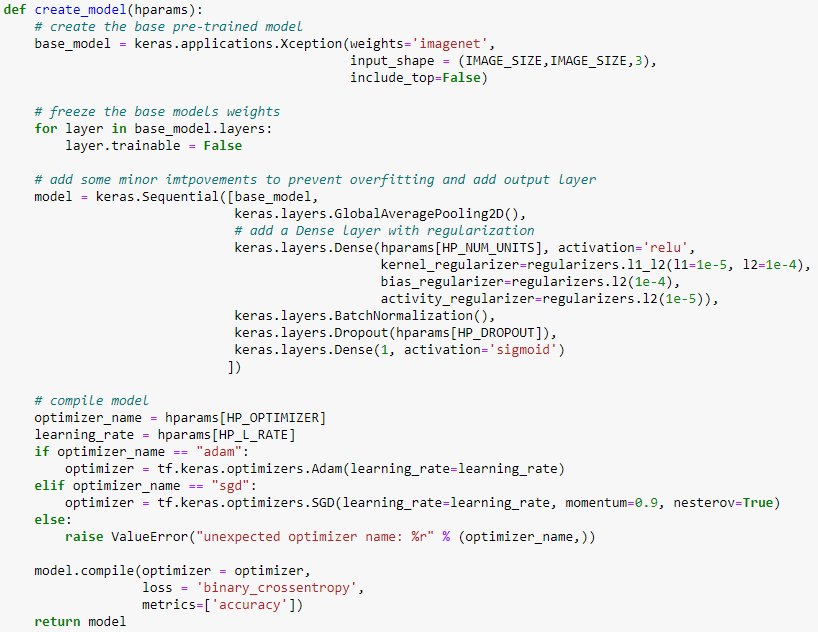
\includegraphics[width=\textwidth]{figures/xception-improvement-1.png}
    \caption{Freezing the base models trainable weights.}
    \label{fig:xception-improvement-1}
\end{figure}
\begin{figure}[H]
    \centering
    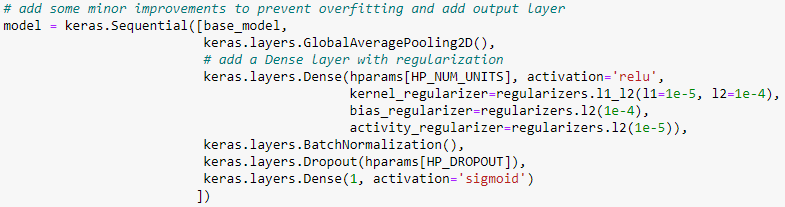
\includegraphics[width=\textwidth]{figures/xception-improvement-2.png}
    \caption{Adding regularisers to the Dense layer.}
    \label{fig:xception-improvement-2}
\end{figure}
\begin{figure}[H]
    \centering
    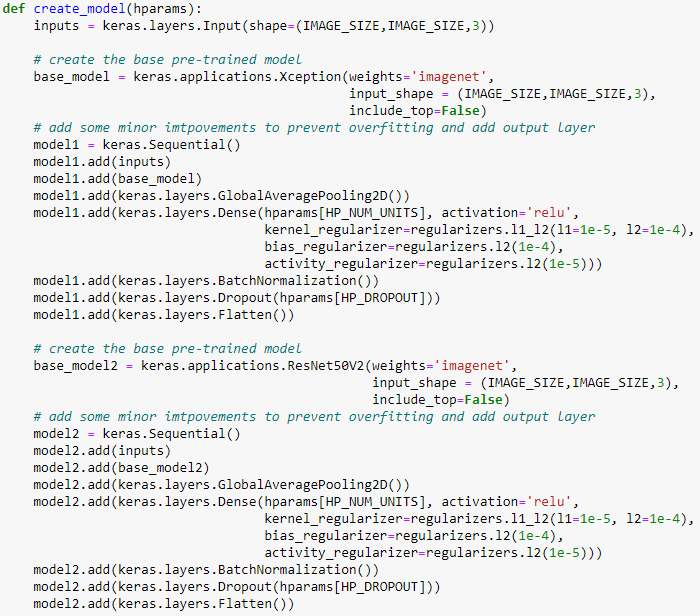
\includegraphics[width=\textwidth]{figures/xception-improvement-3-part1.png}
    \caption{The first half of the Xception-ResNet50V2 model.}
    \label{fig:xception-improvement-3-part1}
\end{figure}
\begin{figure}[H]
    \centering
    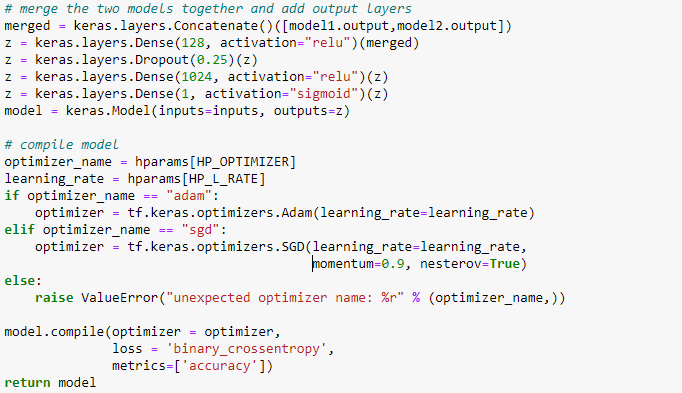
\includegraphics[width=\textwidth]{figures/xception-improvement-3-part2.png}
    \caption{The second half of the Xception-ResNet50V2 model.}
    \label{fig:xception-improvement-3-part2}
\end{figure}
\begin{figure}[H]
    \centering
    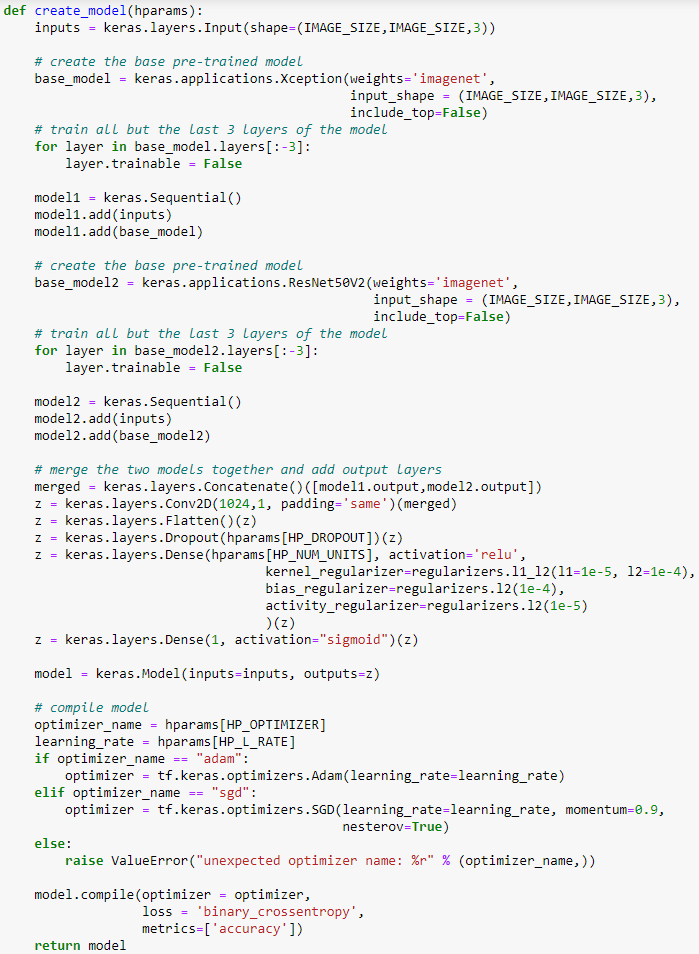
\includegraphics[width=\textwidth]{figures/xception-improvement-4.png}
    \caption{The second version of the Xception-ResNet50V2 model.}
    \label{fig:xception-improvement-4}
\end{figure}
\begin{figure}[H]
    \centering
    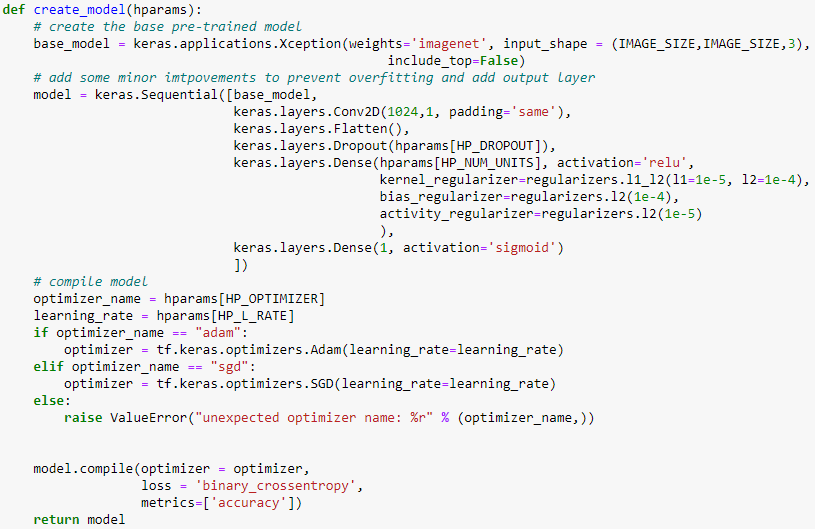
\includegraphics[width=\textwidth]{figures/xception-improvement-5.png}
    \caption{The final improvement to the Xception model.}
    \label{fig:xception-improvement-5}
\end{figure}

\begin{landscape}
\begin{table}
    \caption{Xception improvements results after training on the small COVIDx-CXR dataset.}
    \centering
    \begin{tabular}{l|l|l|l|l|l|l|l|l}
    Model & Optimiser & \begin{tabular}[c]{@{}l@{}}Mean \\ Validation \\ Accuracy\end{tabular} & \begin{tabular}[c]{@{}l@{}}Mean Test\\  Accuracy\end{tabular} & \begin{tabular}[c]{@{}l@{}}Best Fold \\ Test \\ Accuracy\end{tabular} & \begin{tabular}[c]{@{}l@{}}Mean Test\\ Precision\end{tabular} & \begin{tabular}[c]{@{}l@{}}Mean Test\\ Recall\end{tabular} & \begin{tabular}[c]{@{}l@{}}Mean Test\\ F1 Score\end{tabular} & \begin{tabular}[c]{@{}l@{}}Mean \\ Training\\ Time (s)\end{tabular} \\ \hline\hline
    Improvement 1 & Adam  & 0.6827 & 0.5740 & 0.6325 & 0.7293 & 0.2780 & 0.3600 & 177 \\
    Improvement 1 & \begin{tabular}[c]{@{}l@{}}SGD \& \\ Momentum\end{tabular} & 0.6180 & 0.5330 & 0.6225 & 0.5903 & 0.1510 & 0.2241 & 187 \\
    Improvement 2 & Adam & 0.9527 & 0.9395 & 0.9800 & 0.9837 & 0.8950 & 0.9331 & 1132 \\
    Improvement 2 & \begin{tabular}[c]{@{}l@{}}SGD \& \\ Momentum\end{tabular} & 0.9253 & 0.8670 & 0.8975 & 0.9316 & 0.7920 & 0.8555 & 1200 \\
    Improvement 3 & Adam & 0.9407 & 0.9095 & 0.9775 & 0.9864 & 0.8310 & 0.8915 & 1389 \\
    Improvement 4 & Adam & 0.9465 & 0.8240 & 0.9325 & 0.7787 & 0.6660 & 0.7177 & 646 \\
    Improvement 5 & Adam & 0.7180 & 0.6715 & 0.9375 & 0.6826 & 0.5590 & 0.5161 & 922
    \end{tabular}
    \label{fig:xception-improvement-results}
\end{table}
\end{landscape}

\begin{figure}
    \centering
    \begin{subfigure}[b]{0.49\textwidth}
        \centering
        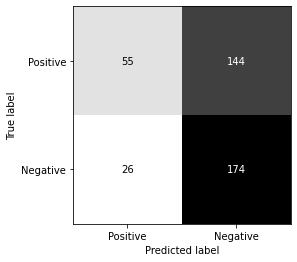
\includegraphics[width=\textwidth]{figures/cm-improv-1.png}
        \caption{Improvement 1 - Adam}
        \label{fig:cm-improv-1}
    \end{subfigure}
    \hfill
    \begin{subfigure}[b]{0.49\textwidth}
        \centering
        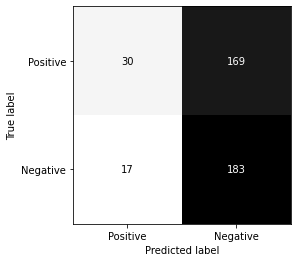
\includegraphics[width=\textwidth]{figures/cm-improv-1-sgd.png}
        \caption{Improvement 1 - Momentum \& SGD}
        \label{fig:cm-improv-1-sgd}
    \end{subfigure}
    \vspace{10mm} %10mm vertical space
    
    \begin{subfigure}[b]{0.49\textwidth}
        \centering
        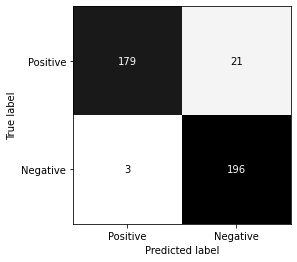
\includegraphics[width=\textwidth]{figures/cm-improv-2.png}
        \caption{Improvement 2 - Adam}
        \label{fig:cm-improv-2}
    \end{subfigure}
    \hfill
    \begin{subfigure}[b]{0.49\textwidth}
        \centering
        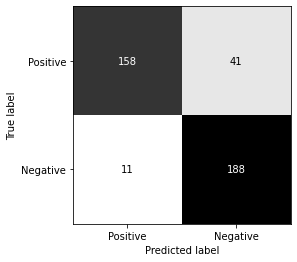
\includegraphics[width=\textwidth]{figures/cm-improv-2-sgd.png}
        \caption{Improvement 2 - Momentum \& SGD}
        \label{fig:cm-improv-2-sgd}
    \end{subfigure}
    \caption{Confusion matrices for the Xception model improvements - Part 1.}
    \label{fig:cm-improv-p1}
\end{figure}
\begin{figure}
    \centering
    \begin{subfigure}[b]{0.49\textwidth}
        \centering
        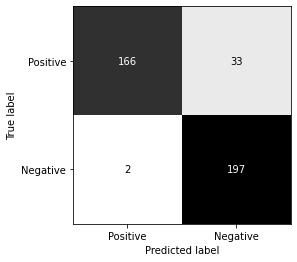
\includegraphics[width=\textwidth]{figures/cm-improv-3.png}
        \caption{Improvement 3}
        \label{fig:cm-improv-3}
    \end{subfigure}
    \hfill
    \begin{subfigure}[b]{0.49\textwidth}
        \centering
        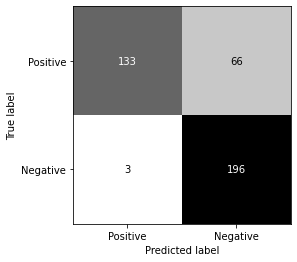
\includegraphics[width=\textwidth]{figures/cm-improv-4.png}
        \caption{Improvement 4}
        \label{fig:cm-improv-4}
    \end{subfigure}
    \vspace{10mm} %10mm vertical space
    
    \begin{subfigure}[b]{0.49\textwidth}
        \centering
        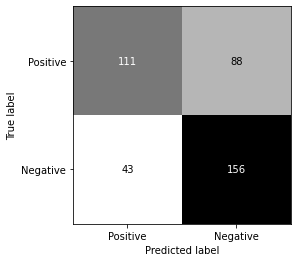
\includegraphics[width=\textwidth]{figures/cm-improv-5.png}
        \caption{Improvement 5}
        \label{fig:cm-improv-5}
    \end{subfigure}
    \caption{Confusion matrices for the Xception model improvements - Part 2.}
    \label{fig:cm-improv-p2}
\end{figure}